\documentclass[13pt]{scrartcl}
\usepackage[utf8]{inputenc}
\usepackage[spanish]{babel}
\usepackage{graphicx}
\usepackage[backend=biber,style=alphabetic]{biblatex}
\usepackage{hyperref}
\hypersetup{
	colorlinks=true,	% false: boxed links; true: colored links
	linkcolor=black,	% color of internal links
	urlcolor=cyan		% color of external links
}
\renewcommand{\familydefault}{\sfdefault}

%opening
\titlehead{Universidad de Granada - Centro de Promoción de Empleo y Prácticas}
\title{Memoria de Prácticas de Empresa - Synergy Movement Technologies 3000 S.L.}
\author{Adrián Morente Gabaldón}
\date{Curso 2017-2018}

\begin{document}
	\maketitle
	
	\begin{center}
		
\includegraphics[scale=0.5]{images/logougr.png}
	\end{center}
	
	\newpage
	\tableofcontents
	\newpage
	
	\section{Introducción}
		Este documento engloba la memoria de prácticas relacionada con las realizadas en la empresa \textit{\textbf{SYMOTECH} (Synergy Movement Technologies 3000 S.L.)}, entre diciembre de 2017 y febrero del 2018. Dicha empresa, dadas sus necesidades, nos ofreció contrato hasta a cinco estudiantes del Grado en Ingeniería Informática; permitiéndonos trabajar en grupo y de forma autónoma, además de aprender y coger experiencia en diferentes sectores de la informática satisfaciendo las distintas tareas necesarias.
		
		La duración de dicho contrato fue de 300 horas (es decir, 5 horas diarias de lunes a viernes, con horario totalmente flexible a nuestra disponibilidad, por condición de estudiantes). Por mi parte, cabe decir que la empresa me ofreció un contrato a tiempo parcial al finalizar dichas prácticas, y a junio de 2018 sigo con ellos en su plantilla.
	
	\section{Descripción de la entidad donde realizó las prácticas}
	
		\subsection{Actividad laboral a la que se dedica la entidad}
			Symotech es una empresa pequeña situada en Granada que desarrolla y comercializa sus dispositivos \textbf{DYNAsystem}. Se tratan de unas estaciones multifuncionales orientadas al rendimiento deportivo y al tratamiento fisioterapéutico, que concentran la mayoría de los modos de entrenamiento que encontramos en un gimnasio, embebidos en forma de ``caja negra'' y con un factor de forma fácilmente integrable en cualquier entorno.
			
			\begin{center}
				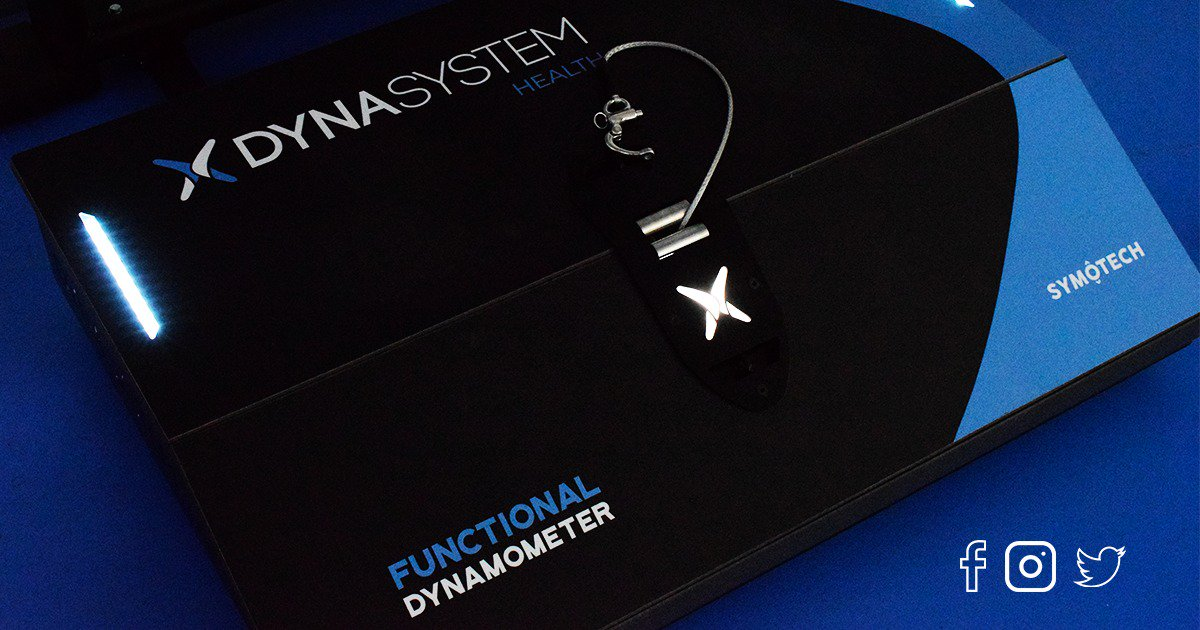
\includegraphics[scale=0.22]{images/dynasystem-blue-floor.jpeg}\\
				DYNASYSTEM HEALTH - imagen corporativa alojada en \href{https://twitter.com/dynasystem_}{Twitter}
			\end{center}
			
			Además, dada la naturaleza electrónica de estos dispositivos, tienen la capacidad de mostrar en tiempo real los datos que se están produciendo por el usuario (como las fuerzas media y máxima, velocidades media y máxima, trabajo, número de repeticiones, tiempo de entrenamiento, etc.). Por otro lado, el control de dicho dispositivo se realiza a través de una aplicación embebida con interacción táctil, desde la que se configuran todos los ejercicios y rutinas deseadas por el usuario.
			
			\begin{center}
				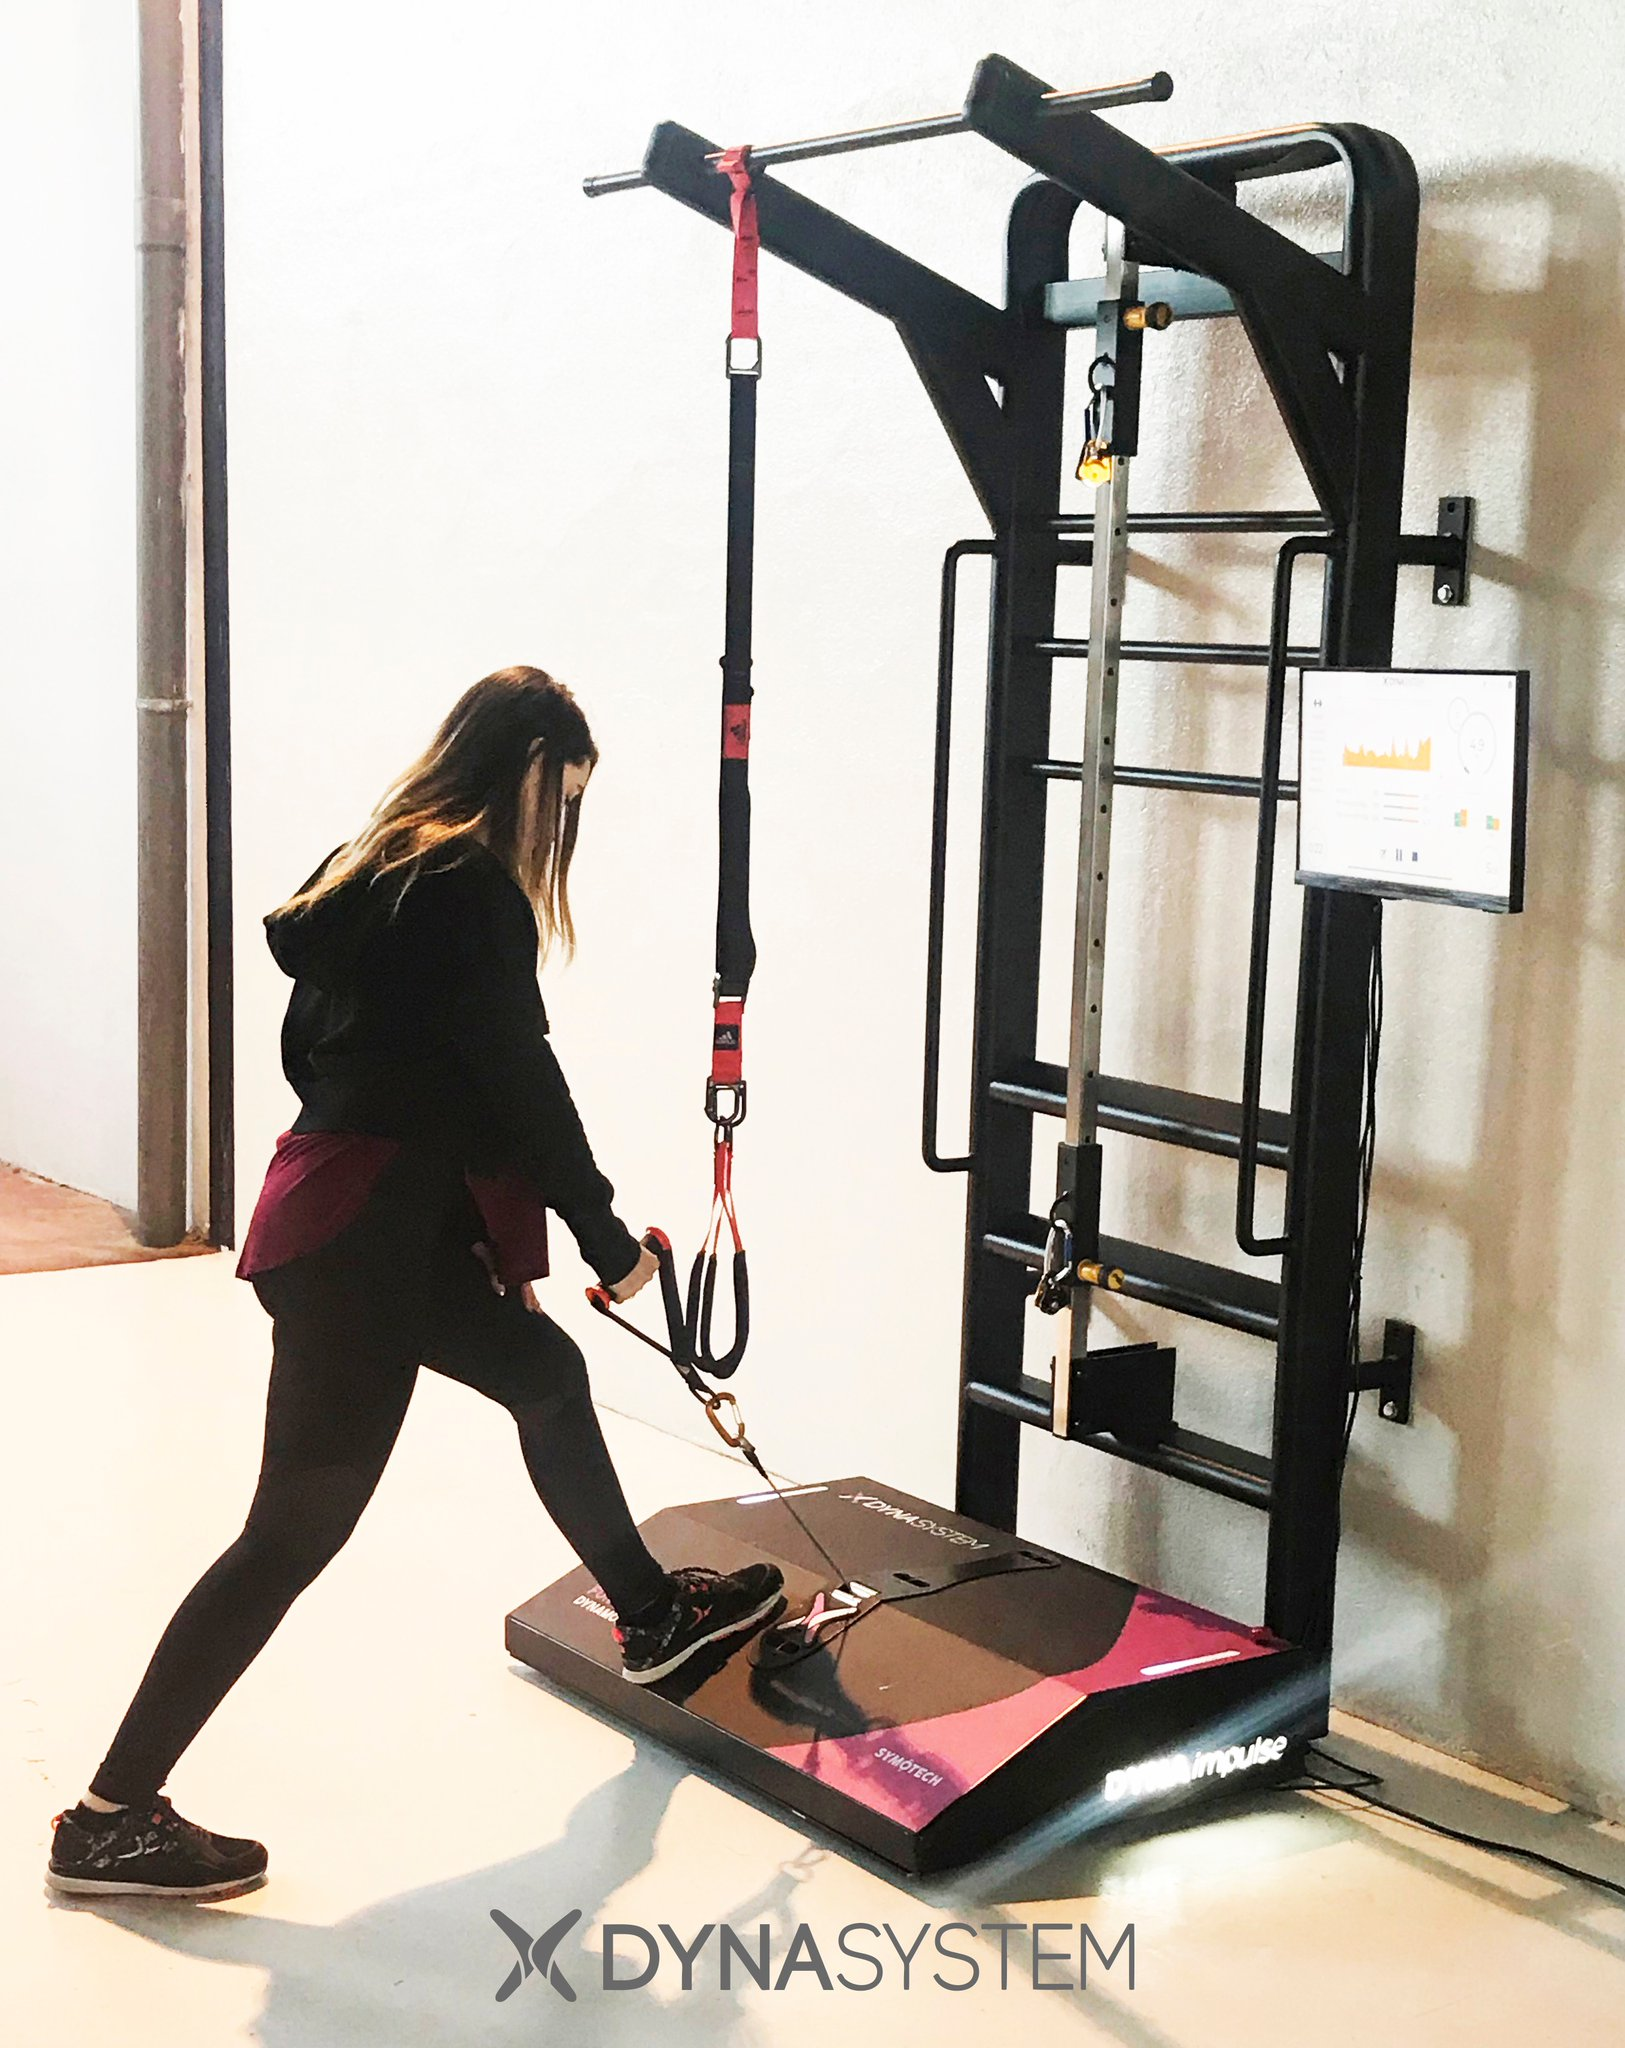
\includegraphics[scale=0.16]{images/dynasystem-pink-station.jpeg}\\
				DYNASYSTEM SPORT - imagen corporativa alojada en \href{https://twitter.com/dynasystem_}{Twitter}
			\end{center}
		
		\subsection{Personal cualificado tecnológicamente de que dispone}
			Como decíamos antes, se trata de una empresa pequeña que dispone de pocos empleados. Entre ellos, encontramos a dos ingenieros electrónicos, a un ingeniero industrial y a dos expertos en ciencias del deporte y fisioterapia. Los estudiantes que entramos a realizar las prácticas con la compañía comportábamos toda la plantilla de informáticos trabajando allí, por lo que pudimos poner en práctica tareas de autogestión y \textit{``brainstorming''} para las labores preestablecidas. Sin embargo, uno de los ingenieros electrónicos, dada su experiencia laboral y su conocimiento de programación, actuó como coordinador de dichas tareas para nosotros.
		
		\subsection{Dotación tecnológica de la que dispone}
			Dado el volumen actual de la empresa, se sitúan en un local mediano con el espacio suficiente para el desarrollo y montaje de dichos dispositivos. Cada uno de los ya empleados en la compañía utilizaban un equipo concedido por la empresa, pero al inicio de las prácticas, cada estudiante trabajaba con su propio equipo portátil, aunque a quien manifestó la necesidad de un equipo informático para trabajar se le concedió rápidamente y sin problema. Sin ir más lejos, yo mismo solicité un equipo de sobremesa potente para realizar las compilaciones del sistema operativo \textit{(del que hablaremos más adelante)} que me fue prestado sin problema.\\
			
			Además, todo el equipo de desarrollo dispusimos de varias unidades de \textit{Raspberry Pi} para las pruebas, tanto de sistema operativo como de aplicación; así como un prototipo de máquina DYNAsystem dedicada solo para nuestras pruebas.\\
			
			En cuanto a conectividad y comunicación, la empresa dispone de conexión de fibra óptica de alta velocidad, por lo que cualquier labor que necesite conexión se hace mucho más cómoda y rápida.
	
	\section{Trabajo realizado}
	
		\subsection{Problemas que se han planteado}
			Al principio del período contractual se nos plantearon las ideas comerciales de la compañía, que nosotros tuvimos que analizar y, en función de los requisitos planteados, proponer soluciones razonables y factibles. Las tareas planteadas fueron las siguientes:
			\begin{itemize}
				\item Diseño, desarrollo y despliegue de una página web estática \textit{(landing)} promocional para el producto, que sustituyese a la entonces vigente. Debía ser sencilla pero elegante, e incluir tanto contenido multimedia útil e ilustrativo, como un formulario de contacto con la empresa.
				\item Análisis, diseño y desarrollo de una aplicación embebida comunicada con la electrónica interna del dispositivo, para controlar mediante interacción táctil el sistema y visualizar los resultados en tiempo real.
				\item Análisis, diseño y desarrollo de una infraestructura embebida que mantuviese y ejecutase dicha aplicación (esto es, cualquier tipo de sistema operativo que satisficiese dicho requerimiento). Entre los requisitos más importantes se encontraban:
					\subitem \textbf{Seguridad}: dado que esta aplicación sería lo único que debía tocar el usuario, era sumamente importante impedir cualquier acceso al sistema operativo, ya fuera mediante teclado o por conexión \textit{SSH (Secure SHell)}, dado que la máquina contiene puertos USB y conectividad WiFi.
					\subitem \textbf{Rapidez}: el usuario espera que la máquina esté encendida y lista para funcionar lo antes posible, así que dicha infraestructura debía ser ligera y con lo mínimo para trabajar; poniendo toda la atención en la \textbf{disponibilidad}.
					\subitem \textbf{Bajos coste y consumo}: dado que este producto era una re-formulación del comercializado por la empresa anterior a Symotech, se pretendía poner solución a errores de estimación e implementación pasados. Uno de estos era el análisis de rendimiento necesario para la aplicación antes mencionada. Veremos en el apartado 3.2.2 la solución planteada para este problema.
			\end{itemize}
			Afortunadamente, la empresa nos brindó total libertad a la hora de elegir proyectos a los que dedicar nuestro tiempo de prácticas. Yo personalmente, decidí dedicarme a la parte de la página web junto con otro compañero, y después de forma autónoma a la infraestructura que mantuviese la aplicación embebida; mientras que el resto de compañeros se dedicaron a la implementación de dicha aplicación. Hablemos de ello en el siguiente apartado.
		
		\subsection{Soluciones que se han llevado a cabo}
			Dado el volumen de cada uno de los problemas y, dado que accedíamos cinco estudiantes a dichas prácticas, optamos inteligentemente y de acuerdo con la empresa a repartirnos las tareas de forma modular. Veamos las labores que desempeñé ordenadas en el tiempo:
			
			\subsubsection{Desarrollo del sitio web y migración del alojamiento}
				Por una parte, dado que poseía algunas habilidades de diseño web que había adquirido por mi cuenta, además de haber recibido clases de asignaturas relacionadas, opté por tomar parte en el diseño de la \textit{landing} junto con otro compañero. Se trataba de un proyecto realmente sencillo, no era necesaria ninguna configuración del \textit{back-end} ni ningún acceso a una base de datos. Dado esto, no era necesario usar más que algún \textit{framework} sencillo de estilo \textit{CSS (Cascading Style Sheet)} como \href{https://www.w3schools.com/w3css/}{W3.CSS}.\\
				
				El mayor interés que nos suscitaba dicha librería se debía a la cantidad de contenedores auxiliares y de ayuda al posicionamiento que contiene. Dado el volumen de clases \textit{CSS} del que dispone, nos permitió realizar un rápido desarrollo de una página totalmente adaptable a cualquier pantalla (tanto escritorio como dispositivo móvil).\\
				
				Dados los ejemplos incluidos en dicha librería, también nos resultó fácil implementar \textit{parallax} en toda la página web; ese efecto visual tan concreto en el que las imágenes permanecen quietas al fondo del \textit{viewport} mientras que el resto del contenido (texto, rectángulos, etc.) se mueven por delante de ellas.\\
				
				A continuación, veamos algunas capturas con parte del contenido de dicho sitio web:
				
				\begin{center}
					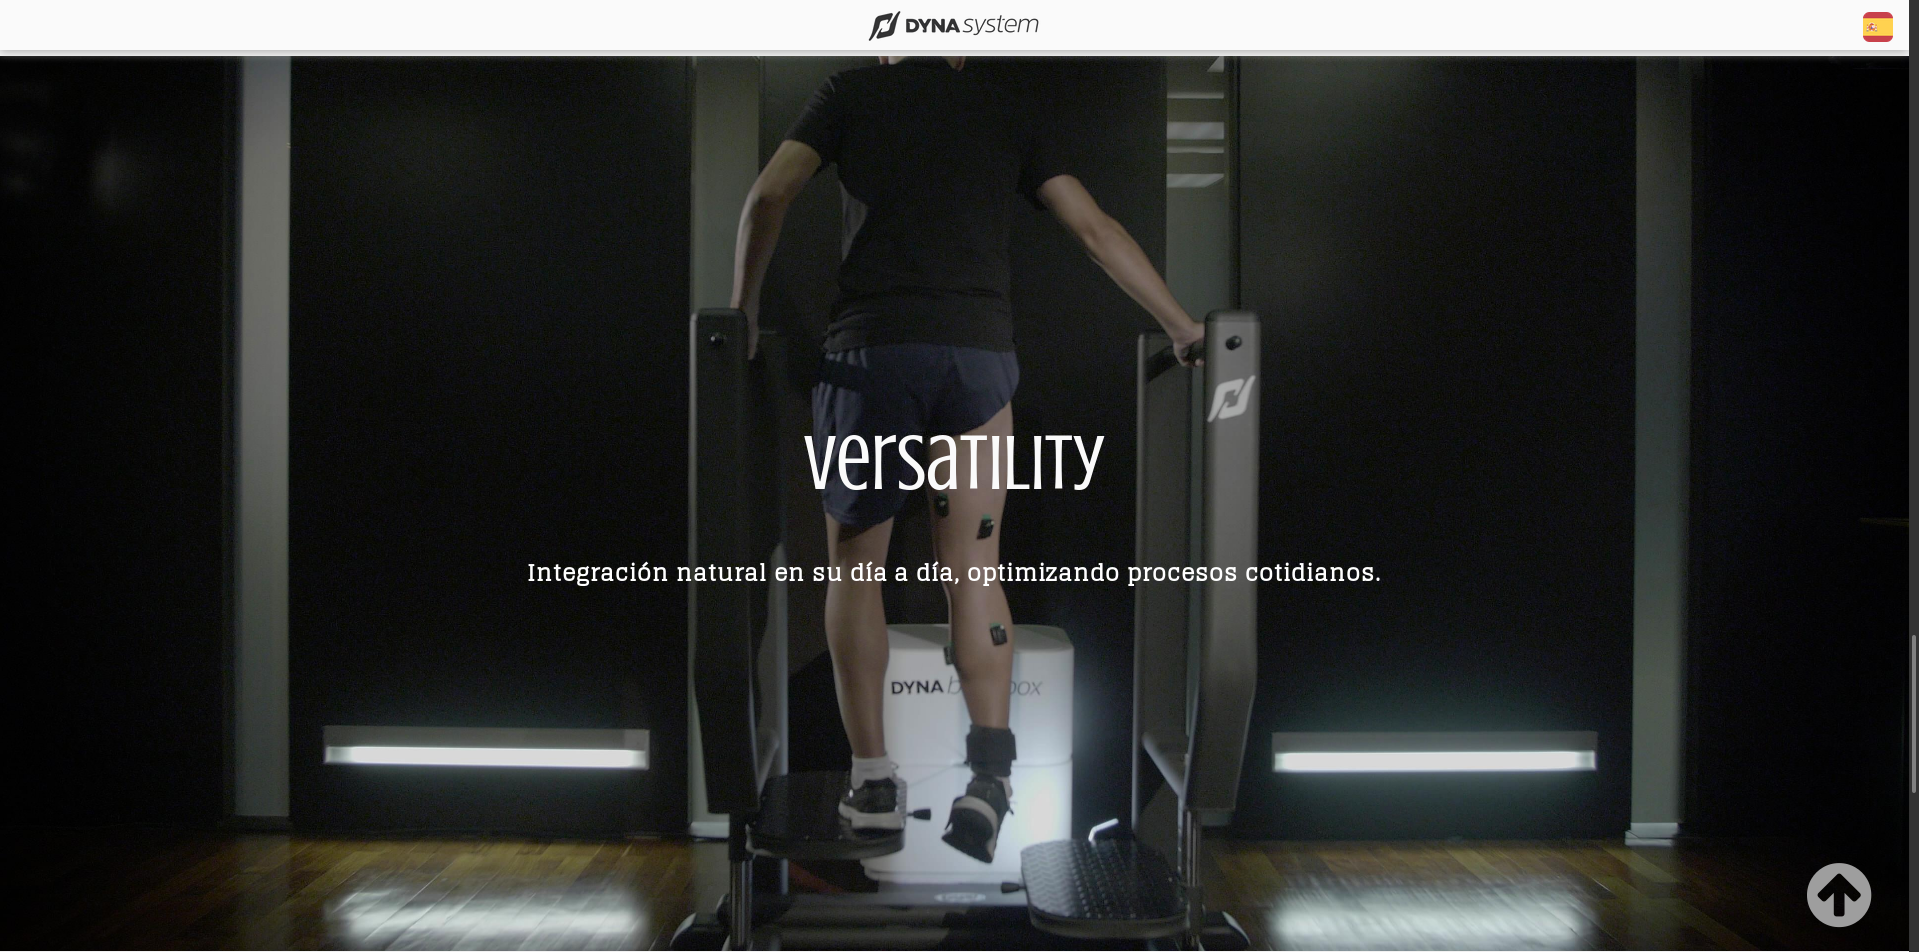
\includegraphics[scale=0.2]{images/web-parallax-screenshot.png}\\
					Captura a pantalla completa de una parte de la web - \href{https://www.dynasystem.es}{dynasystem.es}
				\end{center}
			
				Además, el formulario de contacto estaba implementado en un código PHP de pocas líneas, y en cuanto a visualización tenía el siguiente aspecto:
				
				\begin{center}
					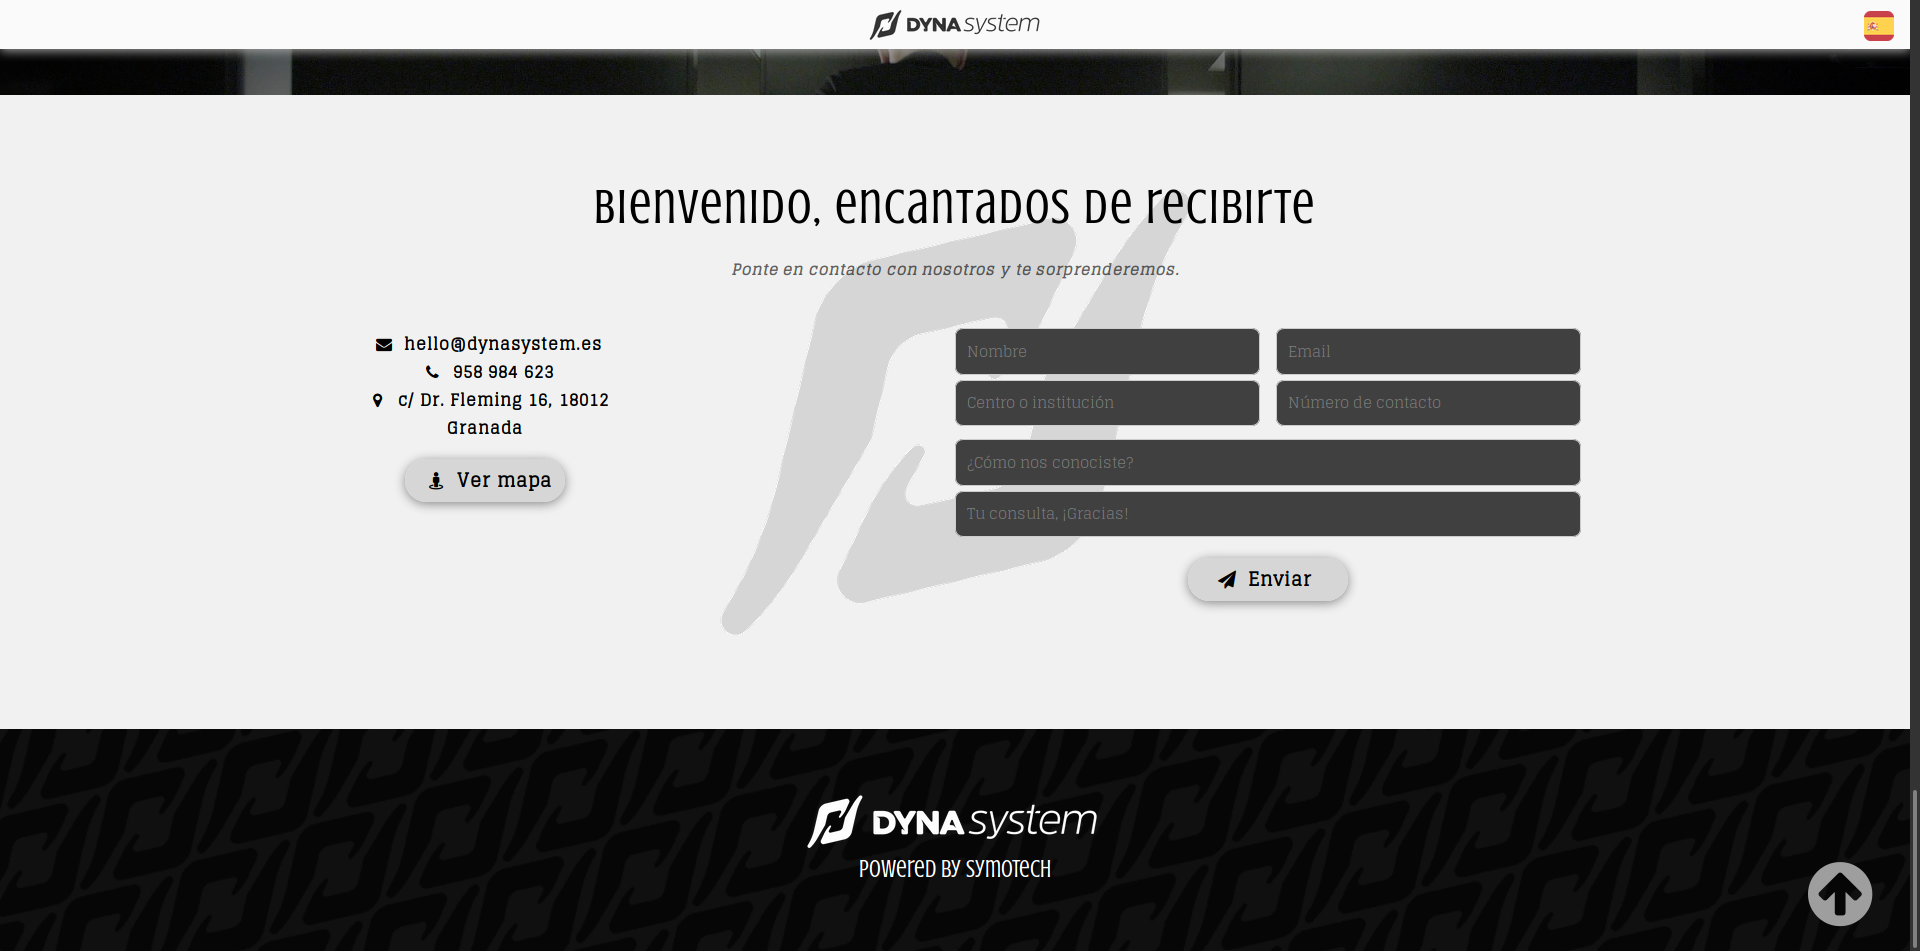
\includegraphics[scale=0.2]{images/web-form-screenshot.png}\\
					Captura a pantalla completa del pie de la página. Muestra los datos de contacto de la empresa, un formulario de contacto y el \textit{footer} personalizado - \href{https://www.dynasystem.es}{dynasystem.es}
				\end{center}
			
				Dicho formulario simplemente cogía los datos introducidos en los campos (validados mediante \textit{Javascript}) y los enviaba por correo electrónico a una de las direcciones de correo corporativas.
			
				\noindent\rule{\textwidth}{0.4pt}\\
				
				Otra parte interesante de dicho desarrollo consiste en \textbf{soporte multilenguaje} del sitio web. Para mayor visibilidad del producto, la compañía estaba interesada en tener una versión del contenido en inglés (y en un futuro, en un abanico más amplio de lenguajes).\\
				
				Sin embargo, como se trataba de una página web estática y no disponíamos de acceso al código de la aplicación servidora, no podíamos generar este contenido de forma dinámica desde dicho código, así que optamos por replicar el archivo \texttt{index.html} escribiendo los textos de dicho fichero en inglés. La interfaz de usuario muestra un botón con una bandera de España que, al ser pulsado, redirige hacia el fichero \texttt{.html} en inglés y con dicho botón mostrando una bandera de Reino Unido.
				
				\noindent\rule{\textwidth}{0.4pt}\\
			
				Por otro lado, una parte importante de dicha tarea fue \textbf{la decisión de la migración del alojamiento}. Cuando llegamos a la empresa, se me autorizó con total transparencia a acceder (con usuario y contraseña) a la plataforma con quien estaba contratado el alojamiento, para poder tener acceso a los servidores SSH y SFTP (necesarios para la actualización del sitio web) además de a los datos de facturación vigentes.\\
				
				Al acceder, vi que la empresa anterior a SYMOTECH había dejado abiertos algunos contratos ahora en desuso, así que opté por sugerir a la compañía el cierre de estos contratos inútiles y la contratación del \textit{hosting} con otro proveedor, ya que la diferencia de precio era grande con respecto al entonces vigente. Los responsables me dieron ``luz verde'' al respecto así que procedimos, y tras el desarrollo de la web, la alojamos en el recién contratado hosting.\\
				
				Para terminar, cabe decir que dicho sitio web ha estado público hasta mediados de junio de 2018, dado que la empresa está pasando por un \textit{rebranding} que atañe tanto a las imágenes de la compañía como a las del producto, y por tanto no se quería mantener la visualización antigua. Sin embargo, se puede obtener \href{https://web.archive.org/web/20180420040111/https://www.dynasystem.es/}{una visualización del 20 de abril a través de la conocida herramienta Web Archive}.

			\subsubsection{Sistema operativo embebido para mantener la aplicación de interfaz táctil}
				Durante las primeras reuniones con los empleados de la compañía, discutimos las tareas y llegamos a la conclusión de que una de ellas era proveer al dispositivo de una infraestructura que mantuviese en ejecución a la aplicación embebida que lo controla, implementando las medidas de seguridad y requisitos de rendimiento que comentamos en el apartado anterior.\\
				
				Vistos los requerimientos de rendimiento y consumo, el ingeniero electrónico coordinador de nuestras prácticas planteó la posibilidad de utilizar \textbf{un ordenador de placa reducida} (en inglés: \textit{Single Board Computer} o \textit{SBC}), como lo son la conocida \textit{Raspberry Pi}, la \textit{Asus Tinkerboard} u otras como la gama \textit{i.MX} del fabricante \textbf{NXP}. La ventaja de usar este tipo de computadores en 2017-2018 es el avance tecnológico que aportan a tan reducido precio, ya que a día de hoy llegan a incluir pequeñas tarjetas gráficas, distintos protocolos de comunicación (como \textit{USB} o \textit{GPIO (General Purpose Input/Output)}) y hasta adaptadores de red inalámbricos (para estándares Wifi y Bluetooth).\\
				
				Dados mi interés y mi experiencia con los sistemas operativos GNU/Linux, planteé la posibilidad de crear nuestra propia distribución UNIX \textit{``desde cero''} con todo lo mínimo para funcionar, a salvedad de alguna customización deseada por nuestra parte. Es cierto que ya existen sistemas operativos orientados a este tipo de dispositivos (como \textit{Raspbian}, el único oficial, o \textit{Snappy Ubuntu Core}, \textit{OSMC} y \textit{LIBREELEC}); pero mientras que el primero tiene todo lo necesario (y más), el resto están orientados a usos más específicos (como Smart TVs o centros multimedia en general). El problema de utilizar un sistema operativo completo como Raspbian es que choca con la sencillez que buscábamos de primeras, ya que contiene instaladas y en ejecución más cosas de las que necesitamos, en detrimento del rendimiento y el ahorro de consumo.\\
				
				Visto esto, comencé a buscar alternativas para crear distribuciones de sistemas operativos basados en Unix, encontrándome principalmente (como opciones mayores) con \textbf{el Proyecto Yocto} y \textbf{Buildroot}. Tras probar ambas, decidí desestimar el uso de \textit{Buildroot} dado que disponía de una configuración mucho más sencilla; lo que puede ser tanto positivo como negativo vistas las necesidades del proyecto. \href{https://www.yoctoproject.org/}{\textit{The Yocto Project}} se trata de un proyecto de código abierto en el que han intervenido grandes empresas, existiendo ahora librerías dedicadas para sistemas \textit{Android}, procesadores \textit{Exynos} de \textbf{Samsung}, placas como \textit{Raspberry Pi} y \textit{Arduino}, además de un larguísimo etcétera [se pueden ver todas las librerías (o \textit{layers}, como se llaman en Yocto) \href{layers.openembedded.org}{aquí}]. Además del extenso soporte empresarial, basta con realizar búsquedas específicas sobre configuración de Yocto y de Buildroot para descubrir que la primera alternativa consta de un uso mucho más extendido entre la comunidad de desarrolladores de dispositivos embebidos.\\
				
				Durante unas semanas de las prácticas estuve adecuándome al entorno por mi cuenta, leyendo toda la documentación y manuales de los desarrolladores de Yocto; así como configurando y compilando algunas imágenes de prueba. Más adelante, para seguir las buenas prácticas de programación y generación de sistemas con Yocto, decidí crear un \textit{layer} propio donde alojar toda la personalización, configuración y programas propios necesarios. Además, siguiendo con la licencia de dicho entorno y, de acuerdo con la empresa, la alojé en mi propio perfil de \href{https://github.com/adrianmorente}{\textbf{GitHub}} con el nombre de \href{https://github.com/adrianmorente/meta-dynasystem}{\textbf{meta-dynasystem}}, siguiendo con las nomenclaturas de dichas librerías. En dicho repositorio se encuentran todas las dependencias y parches necesarios, aunque con el tiempo he ido modificando cosas dada mi permanencia dentro de la empresa. He de decir que todos los programas adicionales han sido implementados en forma de \textbf{servicios de systemd}, el conocido gestor de arranque, \textit{demonios} y procesos en Linux, que hace que el proceso de encendido sea mucho más rápido que con \textit{sysvinit}, más convencional a la par que antiguo. Las características que debí implementar a lo largo de las prácticas fueron las siguientes:
				\begin{itemize}
					\item \textbf{Inclusión de las librerías necesarias para la ejecución de la aplicación embebida:} ya que dicha aplicación fue implementada en \textit{Qt}, era imprescindible que el sistema operativo dispusiera de las librerías necesarias para ejecutar programas de este tipo. Además, fue necesario utilizar el plugin \textbf{EGLFS} de la Raspberry para poder ejecutar aplicaciones gráficas de QML en la interfaz táctil.
					\item \textbf{Medidas de seguridad (cierre intencionado):} para impedir que el usuario pueda cerrar la aplicación y tener acceso a la consola de comandos, implementamos un script que se ejecuta en segundo plano comprobando si se conecta un teclado; caso en el que el sistema informa de ello y se reinicia.
					\item \textbf{Medidas de seguridad (cierre involuntario):} en el caso de que la aplicación sufra algún problema y se cierre inesperadamente, el sistema operativo se da cuenta al instante de esto y reinicia la máquina. Esto fue implementado lanzando la aplicación desde un script en lugar de un servicio, de forma que el script es consciente de cuando la aplicación finaliza su ejecución.
					\item \textbf{Pantalla de inicio personalizada:} mientras que el sistema carga el kernel y todo lo necesario para ejecutar a pantalla completa la aplicación, propuse la existencia de una imagen estática en pantalla durante este proceso. Consistió simplemente en coger una aplicación como \textit{PSplash} (soportada inherentemente por Yocto), migrar el proceso del arranque con \textit{sysvinit} a \textit{systemd} (creando un servicio concreto para el mismo y lanzándolo lo antes posible en el sistema) y creando un parche con la imagen deseada:
					
					\begin{center}
						
\includegraphics[width=\linewidth]{images/dynasystem.jpeg}
					\end{center}
					
					\item \textbf{Encendido de la máquina más natural:} esto requiere varios matices. Como dijimos anteriormente, la idea del dispositivo embebido es que el usuario solo se enfrente a la aplicación, sin saber qué hay detrás de ella ni qué infraestructura la soporta (lo que le resultaría más \textit{natural}). Sin embargo, cuando encendemos un ordenador con Linux siempre accedemos a ver un fragmento de terminal mostrando mensajes de la carga del kernel. Además, al iniciar la Raspberry muestra a pantalla completa un arco iris en forma de degradado (esto es para probar que la pantalla funciona), así como su logo durante la carga del kernel. Dicho esto, para que el arranque fuese más natural al usuario, tuve que modificar los ficheros \textbf{/boot/config.txt} y \textbf{/boot/cmdline.txt} para prescindir de estas cosas; de forma que cuando el usuario enciende la máquina, lo primero que ve en la pantalla es la imagen de carga descrita anteriormente.
					\item \textbf{Actualizaciones \textit{OTA}:} esta fue otra característica que propuse al equipo para poder actualizar los dispositivos una vez que estuvieran vendidos e instalados en algún lugar del mundo. Sin embargo, por temas de temporalidad, no pude realizar esta tarea hasta finalizado mi contrato de prácticas.
				\end{itemize}
			
		\subsection{Herramientas utilizadas para llevar a cabo el trabajo realizado}
			Ya hemos mencionado en el desarrollo de las soluciones la mayoría de las herramientas utilizadas durante el trabajo, pero en este apartado detallaremos algunas de ellas, las relacionadas con mi parte, con mayor profundidad. Por otro lado, a nivel de equipo utilizamos herramientas como \textit{Trello} y \textit{Slack}, para gestión de tareas basadas en tableros \textit{kanban} y para comunicación interna, respectivamente.
			
			\subsubsection{Página web}
				Para empezar, hablemos del sitio web antes detallado. Este fue realizado por mi compañero y yo usando los lenguajes de \textit{HTML5} (para toda la estructura del documento), \textit{CSS3} (para el estilo, y usando la librería \textbf{W3.CSS} antes mencionada), Javascript (en el estándar \textit{ES6}, para comportamiento de botones, animaciones, etc.) y finalmente \textit{PHP} para el sencillo formulario de contacto.
				
				Por otro lado, para el desarrollo utilicé \textit{Atom}, por aquel entonces mi editor favorito; así como \textbf{control de versiones} basado en \textbf{git} junto con mi compañero; concretamente, en \textit{Github}. Además, para hacer intercambio de archivos y subir el sitio web a producción utilizamos \textbf{Filezilla}, una cómoda y ligera herramienta \textit{SFTP} de código abierto.
				
			\subsubsection{Sistema operativo}
				Como mencionamos arriba, nos basamos en el proyecto \textit{Yocto}, que a su vez aúna las herramientas de \textbf{OpenEmbedded}, proyecto inicial del que deriva el primero. A su vez, se basan en los lenguajes \textit{Python} y \textit{Bitbake} para su desarrollo, mientras que el segundo es el utilizado para la configuración y el \textit{tweaking} de los sistemas operativos generados.\\
				
				Como dijimos previamente, también fue necesario instalar en dicho sistema las librerías de \textit{Qt}; además de lo cual opté por poner a punto un sistema de compilación cruzada para generar en el propio ordenador de sobremesa ejecutables compatibles con la arquitectura de la Raspberry Pi. Esto se hizo pensando en que mis compañeros pudieran realizar las pruebas de su aplicación sobre mi versión temprana del sistema operativo en dicha placa, mientras que yo proseguía con otras tareas.\\
				
				Por otro lado, las herramientas más básicas utilizadas fueron la terminal (prácticamente todo el tiempo, dada mi habilidad con ella para administrar sistemas y la comodidad que me transmite a la hora de controlar cualquier cosa, desde realizar un commit a \textit{Github} hasta crear un fichero plano), \textit{git} y un amplio abanico de comandos de Linux. Para terminar, utilicé la herramienta \href{https://etcher.io}{etcher.io} para instalar en las tarjetas de memoria los sistemas operativos generados.\\
				
				Por otro lado, Yocto provee de un plugin para el entorno de desarrollo integrado \textit{Eclipse}, pero dicho entorno en Linux aporta más complicación en su sola instalación que la que da cualquier editor sencillo junto con una terminal, así que opté por la segunda alternativa.

		\subsection{Asignaturas de la titulación que hayan resultado útiles para llevar a cabo el trabajo realizado}
			Aunque cualquier asignatura a lo largo de la carrera es ilustrativa a la hora de pensar como un ingeniero técnico en informática en formación, algunas de las asignaturas que fueron más útiles durante el trabajo son las siguientes:
			
			\begin{itemize}
				\item \textbf{Página web:} resultaron de utilidad \textit{Tecnologías Web (TW)} y \textit{Desarrollo de Aplicaciones para Internet(DAI)}. \textit{TW} fue la primera asignatura de diseño web que cursé en la carrera, y enfoca todos los fundamentos de las páginas a un punto más básico, reduciendo todo lo que vemos a un sencillísimo modelo de cajas, que implementado de forma ordenada facilita mucho el desarrollo y el posicionamiento de todos los componentes necesarios para mostrar la información. Por otro lado, \textit{DAI} da por sabidos dichos fundamentos y muestra un punto más ilustrativo para la separación entre \textit{cliente} y \textit{servidor}, muy útil a la hora de optimizar los recursos alojados en una página estática (o de cualquier tipo).
				\item \textbf{Sistema operativo:} resultaron de utilidad tanto \textit{Sistemas Operativos (SO)} como \textit{Ingeniería de Servidores (ISE)}. La primera sirvió para iniciación avanzada a la línea de comandos, una actividad que he explotado mucho a lo largo de la carrera y que me empujó a interesarme aún más por los sistemas Linux y sus fundamentos. Por otro lado, \textit{ISE} fue de gran utilidad para la administración de sistemas (ya sean orientados a servidores o a sistemas operativos autónomos), y que además me resultó de gran interés visto el que ya tenía por dichas actividades.
			\end{itemize}
	
	\section{Bibliografía utilizada}
		Entre la bibliografía utilizada de carácter general, se encuentra la siguiente lista:
		
		\begin{itemize}
			\item Manual de Cascading StyleSheet - \href{https://www.w3schools.com/css/default.asp}{w3schools.com CSS Tutorial}
			\item W3.CSS Faster and better fully responsive CSS - \href{https://www.w3schools.com/w3css/default.asp}{w3schools.com W3.CSS}
			\item Manual de iniciación rápida a Yocto Project - \href{https://www.yoctoproject.org/docs/2.5/brief-yoctoprojectqs/brief-yoctoprojectqs.html}{Yocto Project Quick Build}
			\item Manual completo avanzado de Yocto Project - \href{https://www.yoctoproject.org/docs/2.4/mega-manual/mega-manual.html}{Yocto Project Mega-Manual}
			\item Utilidad para formatear dispositivos de memoria con imágenes de sistema - \href{https://etcher.io}{etcher.io}
			\item Inclusión de librerías Qt5 en Yocto - \href{http://wiki.dh-electronics.com/index.php?title=Building_Qt5_using_Yocto}{Building Qt5 using Yocto - DH electronics}
			\item Compilación cruzada de Qt - \href{https://wiki.qt.io/RaspberryPi2EGLFS}{RaspberryPi2EGLFS}
			\item Foro de Raspberry Pi (configuración del dispositivo) - \href{https://www.raspberrypi.org/forums/}{Raspberry Pi Forums}
			\item Comunidad NXP Solutions (configuración de Yocto para dispositivos embebidos) - \href{https://community.nxp.com/}{NXP Solutions forums}
			\item Compilación de imagen de ejemplo de Yocto para Raspberry Pi - \href{http://www.jumpnowtek.com/rpi/Raspberry-Pi-Systems-with-Yocto.html}{Building Raspberry Pi Systems with Yocto}
			\item Otro ejemplo de compilación de imagen rápida de Yocto - \href{https://medium.com/@shigmas/yocto-pi-and-qt-e9f2df38a610}{Yocto, Pi and Qt}
		\end{itemize}
	
		Por otro lado, hice buen provecho de foros de gran volumen como Stack Overflow, dado que muchos usuarios de Yocto realizan preguntas muy específicas al toparse con un problema, y gente las resuelve sin llegar a redactar ningún artículo extenso al respecto.
	
	\section{Valoración personal del trabajo realizado y conclusiones}
		Personalmente, me siento muy satisfecho con el trabajo realizado. Para empezar, las condiciones que me brindó la empresa fueron sensacionales, empezando por la flexibilidad de horarios y continuando con la importancia de la palabra de cada empleado; dándome ánimos a dar un paso adelante, a pensar en el futuro del proyecto sintiéndome parte de él y a tomar decisiones responsables que lo acompañasen.\\
		
		Además, estos meses de trabajo con la empresa me han servido para aprender un paradigma al que nunca pensaba acercarme. Si bien es cierto que he dicho que Linux me ha gustado desde que empecé la carrera y que desde entonces he tenido soltura con su administración; \textbf{jamás pensé que acabaría diseñando una distribución propia basada en UNIX}. Por si fuera poco, al enfrentarme yo solo a esta tarea, me sentí guía de mí mismo a la hora de idear y estudiar soluciones y/o posibles propuestas. Esto no quiere decir que estuviera solo, ya que antes de proceder tras tomar una decisión la comentaba con el resto del equipo (tanto de estudiantes como los ingenieros electrónicos que nos acompañaban), ya que \textit{cuatro ojos ven más que dos} y cualquiera puede estar equivocado aunque no lo piense.\\
		
		Por otro lado, el período de prácticas de empresa me parecen una experiencia prácticamente obligada para cualquier estudiante del grado, tanto de Ingeniería Informática como de cualquier carrera técnica, y algo que ya he recomendado y que seguiré recomendando a cualquier estudiante que conozca. Independientemente de si al finalizar esta temporada se produce una contratación por parte de la empresa o no, el hecho de enfrentarse a un proyecto real genera mucha madurez tanto personal como profesional. Además de no ya solo la ayuda económica que suponen este y cualquier trabajo, \textbf{la formación vale mucho dinero}; y como estudiante es una etapa indispensable en la que la persona aprende a organizarse en su vida personal para compaginar estudios y empleo, además de entrenarse con la estimación de los intervalos de tiempo necesarios para el desempeño de futuros proyectos.\\
		
		Para terminar, agradezco la oportunidad brindada para seguir en la empresa y formar parte de un proyecto tan interesante sin siquiera haber finalizado el grado.

\end{document}
